% This version of CVPR template is provided by Ming-Ming Cheng.
% Please leave an issue if you found a bug:
% https://github.com/MCG-NKU/CVPR_Template.

%\documentclass[review]{cvpr}
\documentclass[final]{cvpr}

\usepackage{times}
\usepackage{epsfig}
\usepackage{graphicx}
\usepackage{amsmath}
\usepackage{amssymb}

\usepackage{url}            % simple URL typesetting
\usepackage{booktabs}       % professional-quality tables
\usepackage{amsfonts}       % blackboard math symbols
\usepackage{nicefrac}       % compact symbols for 1/2, etc.
\usepackage{microtype}      % microtypography

\usepackage{graphicx}
\usepackage{amsmath,amssymb} % define this before the line numbering.
\usepackage{bbold}
\usepackage{dsfont}
\usepackage{enumerate}
\usepackage[toc,page]{appendix}
\usepackage[font=small,labelfont=bf]{caption}

\usepackage{enumitem}

\usepackage{xcolor}
\usepackage{caption}
\usepackage{subcaption}
\usepackage{bm}
\usepackage{isomath}
\usepackage{arydshln}
\usepackage{stmaryrd}

\usepackage{fixltx2e}
\usepackage{dblfloatfix}
\usepackage{pbox}
\usepackage{capt-of}

\usepackage[normalem]{ulem}
\usepackage{multirow}

\usepackage{colortbl}

\usepackage{mathtools}
\usepackage{array}

\makeatletter
\@namedef{ver@everyshi.sty}{}
\makeatother
\usepackage{pgf}

\newcommand{\xpt}{\edef\f@size{\@xpt}\rm}

\def\ie{\emph{i.e.}}
\def\etc{\emph{etc}}

\usepackage{tikz}

\newcommand{\comment}[1]{}

\usepackage{indentfirst}
% variables
%\vec{\mathcal{M}}
\renewcommand\vec[1]{\ensuremath\boldsymbol{#1}}
\renewcommand\cdots{...}
\newcommand{\tC}{\vec{\mathcal{C}}}
\newcommand{\tH}{\vec{\mathcal{H}}}
\newcommand{\tB}{\vec{\mathcal{B}}}
\newcommand{\tY}{\vec{\mathcal{Y}}}
\newcommand{\tF}{\vec{\mathcal{F}}}
\newcommand{\cB}{\mathcal{B}}
\newcommand{\mB}{\mathbf{B}}
\newcommand{\mY}{\mathbf{Y}}
\newcommand{\mZ}{\mathbf{Z}}
\newcommand{\vb}{\mathbf{b}}
\newcommand{\vy}{\mathbf{y}}
\newcommand{\valpha}{\bm{\alpha}}
\newcommand{\tX}{\vec{\mathcal{X}}}
\newcommand{\cX}{\mathcal{X}}
\newcommand{\mX}{\mathbf{X}}
\newcommand{\vx}{\mathbf{x}}
\newcommand{\mbrp}[1]{\mathbb{R}_{+}^{#1}}
\newcommand{\mbr}[1]{\mathbb{R}^{#1}}
\newcommand{\mbn}[1]{\mathbb{N}^{#1}}
\newcommand{\mbnz}[1]{\mathbb{N}_{0^+}^{#1}}
\newcommand{\mbnp}[1]{\mathbb{N}_{+}^{#1}}
\newcommand{\stackThree}{{;}_{3}}
\newcommand{\vbeta}{\vec{\beta}}
%\newcommand{\rank}[1]{\text{Rank}({#1})}

%\newcommand{\tXS}{\vec{\mathcal{X}}^{*}}
\newcommand{\vv}{\mathbf{v}}
\newcommand{\vq}{\mathbf{q}}
\newcommand{\tV}{\vec{\mathcal{V}}}
\newcommand{\tE}{\vec{\mathcal{E}}}
\newcommand{\tEH}{\vec{\mathcal{\hat{E}}}}
\newcommand{\tVH}{\vec{\mathcal{\bar{V}}}}
\newcommand{\tVT}{\vec{\mathcal{\hat{V}}}}
\newcommand{\idx}[1]{\mathcal{I}_{#1}}
\newcommand{\semipd}[1]{\mathcal{S}_{+}^{#1}}
\newcommand{\spd}[1]{\mathcal{S}_{++}^{#1}}

\newcommand{\tR}{\vec{\mathcal{R}}}
\newcommand{\vu}{\mathbf{u}}
\newcommand{\vup}{\mathbf{u^{'}}}
\newcommand{\vz}{\mathbf{z}}
\newcommand{\vzeta}{\boldsymbol{\zeta}}
\newcommand{\vc}{\mathbf{c}}

\newcommand{\vphi}{\boldsymbol{\phi}}
\newcommand{\vpsi}{\boldsymbol{\psi}}
\newcommand{\tPsi}{\vec{\mathcal{V}}}
\newcommand{\bigoh}{\mathcal{O}}
\newcommand{\mPsi}{\vec{\Psi}}
\newcommand{\vj}{\vec{j}}

% operators
\newcommand{\enorm}[1]{\left\|{#1}\right\|_2}
\newcommand{\fnorm}[1]{\left\|{#1}\right\|_F}
\newcommand{\lnorm}[1]{\left\|{#1}\right\|_1}
\newcommand{\riem}{\mathbf{d}_{\mathcal{R}}}
\newcommand{\spdp}[1]{\mathbb{S}_{++}^{#1}}
\newcommand{\simplex}[1]{\Delta^{#1}}
\newcommand{\set}[1]{\left\{#1\right\}}

\DeclareMathOperator*{\argmin}{arg\,min}
\DeclareMathOperator*{\argmax}{arg\,max}
\DeclareMathOperator*{\supp}{Supp}
\DeclareMathOperator*{\unique}{Unique}
\DeclareMathOperator*{\TRank}{TRank}
\DeclareMathOperator*{\rank}{Rank}
\DeclareMathOperator*{\spann}{Span}
\DeclareMathOperator*{\sym}{Sym}

\newcommand{\flatt}[1]{\text{Flatten}\!\left({#1}\right)}
\newcommand{\unflatt}[1]{\text{Flatten}^{-1}\!\left({#1}\right)}
\newcommand{\myspan}[1]{\spann\left(#1\right)}

\DeclareMathOperator*{\trace}{Tr}
%\DeclareMathOperator*{\rank}{Rank}
\DeclareMathOperator*{\kronstack}{\uparrow\!\otimes}

\DeclareMathOperator*{\avg}{avg}
\DeclareMathOperator*{\sgn}{Sgn}
\DeclareMathOperator*{\hosvd}{HOSVD}
\DeclareMathOperator*{\logm}{Log}
\DeclareMathOperator*{\detm}{Det}
\DeclareMathOperator*{\fg}{g}
\newcommand{\expl}[1]{\text{e}^{#1}}
\DeclareMathOperator*{\res}{Res}
\DeclareMathOperator*{\asinh}{Asinh}
%\newcommand{\exp}[1]{e^{#1}}




\newcommand{\mI}{\mathbf{I}}
\newcommand{\normvec}[1]{\frac{#1}{\|{#1}\|_2}}
\newcommand{\suptensor}[1]{\mathfrak{S}^{#1}}
\newcommand{\suptensorr}[2]{\mathfrak{S}^{#1}_{\times^{#2}}}
\newcommand{\region}{\mathcal{R}}

%\newtheorem{theorem}{Theorem}
%\newtheorem{definition}{Definition}
%\newtheorem{lemma}{Lemma}
%\newtheorem{proposition}{Proposition}
%\newtheorem{remark}{Remark}

\newcommand{\todo}[1]{{\bf \textcolor{red}{[TODO: #1]}}}


\newcommand{\mLa}{\bm{\lambda}^{*}}
\newcommand{\mLambda}{\bm{\lambda}}
\newcommand{\mU}{\bm{U}}
\newcommand{\mV}{\bm{V}}
\newcommand{\timetplone}{{(t+1)}}
\newcommand{\timet}{{(t)}}

\newcommand{\mBOvl}{{\mB^{*}}}

\newcommand{\piA}{{\Pi_A}}
\newcommand{\piB}{{\Pi_B}}

\newcommand{\sigmav}{{^v\!\!\,{\sigma}}}
%\newcommand{\thickhat}[1]{\mathbf{\ddot{\text{$#1$}}}}
\newcommand{\sigmas}{{^s\!\!\,{\sigma}}}

\newcommand{\fvx}{{\boldsymbol{f}(\vx)}}
\newcommand{\fvy}{{\boldsymbol{f}(\vy)}}

\newcommand{\vsss}{\boldsymbol{s}}
\newcommand{\vw}{\boldsymbol{w}}

\newcommand{\vphibar}{\boldsymbol{\bar{\phi}}}
\newcommand{\vsigma}{\boldsymbol{\sigma}}

\def\eg{\emph{e.g.}}

\newcommand{\myg}[1]{\boldsymbol{G}\left(#1\right)}
\newcommand{\mygtwo}[1]{\boldsymbol{G}\Big(#1\Big)}
%\newcommand{\mygthree}[1]{\boldsymbol{G}\left(#1\right)}
\newcommand{\mygthree}[1]{\boldsymbol{\mathcal{G}}\!\left(\!#1\!\right)}
\newcommand{\mygfour}[1]{\boldsymbol{\mathcal{G}}\!\Bigg(\!#1\!\Bigg)}
\newcommand{\tG}{\boldsymbol{\mathcal{G}}}

\newcommand{\vPhi}{\boldsymbol{\Phi}}
\newcommand{\invbeta}{{(1\!-\!\beta)}}
\newcommand{\invsqrtbeta}{\sqrt{1\!-\!\beta}}
\newcommand{\sqrtbeta}{\sqrt{\beta}}


\newcommand{\mIdent}{\boldsymbol{\mathds{I}}}
\newcommand{\sIdent}{\mathds{I}}
\newcommand{\vOnes}{\mathbb{1}}

\newcommand{\mJ}{\mathbf{J}}
\newcommand{\sXkl}{{X_{kl}}}

\newcommand{\mK}{\mathbf{K}}
\newcommand{\mKb}{\bar{\mK}}
\newcommand{\mKbb}{\bar{\mKb}}
\newcommand{\Kb}{\bar{K}}
\newcommand{\Kbb}{\bar{\Kb}}
\newcommand{\mC}{\mathbf{C}}

\newcommand{\mKro}{{\mK^{q}}}
\newcommand{\mKbro}{{\mKb{\,\!}^{q}}}
\newcommand{\mKbbro}{{\mKbb^{q}}}
\newcommand{\Kbro}{{\Kb^{q}}}
\newcommand{\Kbbro}{{\Kbb^{q}}}



\newcommand{\fvxt}{{\boldsymbol{f}^{(t)}(\vx)}}
\newcommand{\Fvxt}{{\boldsymbol{F}^{(t)}(\vx)}}
\newcommand{\fvxtplusone}{{\boldsymbol{f}^{(t+1)}(\vx)}}
\newcommand{\Fvxtplusone}{{\boldsymbol{F}^{(t+1)}(\vx)}}
\newcommand{\vxzero}{\mathbf{x}_0}
\newcommand{\fvxzerotplusone}{{\boldsymbol{f}^{(t+1)}(\vxzero)}}
\newcommand{\Fvxzerotplusone}{{\boldsymbol{F}^{(t+1)}(\vxzero)}}
\newcommand{\fvxzerotplusonei}{{\boldsymbol{f}_i^{(t+1)}(\vxzero)}}

\newcommand{\tFvxt}{{{\vec{\mathcal{F}}}^{(t)}(\vx)}}
\newcommand{\tFvxtplusone}{{{\vec{\mathcal{F}}}^{(t+1)}(\vx)}}
\newcommand{\tFvxzerotplusone}{{{\vec{\mathcal{F}}}^{(t+1)}(\vxzero)}}




\newcommand{\swbar}{\bar{w}}
\newcommand{\vwbar}{\bar{\boldsymbol{w}}}

\newcommand{\vvartheta}{\boldsymbol{\vartheta}}
\newcommand{\tprim}[1]{{\uparrow T_{#1}}}


\newcommand{\vS}{\boldsymbol{S}}

\newcommand{\barM}{{\bar{M}}}
\newcommand{\barmM}{{\bar{\vec{M}}}}

\newcommand{\sN}{\vec{N}}
\newcommand{\tN}{\vec{\mathcal{N}}}
\newcommand{\tP}{\vec{\mathcal{P}}}
\newcommand{\tS}{\vec{\mathcal{S}}}
\newcommand{\tSnb}{\mathcal{S}}
\newcommand{\mS}{\vec{S}}
\newcommand{\tNnb}{\mathcal{N}}

\newcommand{\cov}{\boldsymbol{\Sigma}}
\newcommand{\covb}{\boldsymbol{\Sigma}^{(\!\diamond\!)}}
\newcommand{\covw}{\boldsymbol{\Sigma}^{(\!*\!)}}
\newcommand{\vphix}[1]{{\boldsymbol{\phi}\left({#1}\right)}}
\newcommand{\covbb}[1]{{\boldsymbol{\Sigma}^{(\diamond,{#1})}}}
\newcommand{\covww}[1]{{\boldsymbol{\Sigma}_c^{(*,{#1})}}}

\newcommand{\muw}{\boldsymbol{\mu}^{(*)}}
\newcommand{\mub}{\boldsymbol{\mu}^{(\diamond)}}

\newcommand{\mubb}[1]{{\boldsymbol{\mu}^{(\diamond,{#1})}}}
\newcommand{\muww}[1]{{\boldsymbol{\mu}_c^{(*,{#1})}}}
\newcommand{\muwww}[2]{{\boldsymbol{\mu}_{#1}^{(*,{#2})}}}

\newcommand{\mPhi}{\boldsymbol{\Phi}}
\newcommand{\parsmP}{\!\left(\mPhi\right)}
\newcommand{\parsmPc}{\!\left(\mPhi_c\right)}
\newcommand{\parsmPA}{\!\left(\mPhi^A\right)}
\newcommand{\parsmPB}{\!\left(\mPhi^B\right)}
\newcommand{\parsmPAB}{\!\left(\mPhi^A\!,\mPhi^B\right)}
\newcommand{\parsmPcA}{\!\left(\mPhi_c^A\right)}
\newcommand{\parsmPcB}{\!\left(\mPhi_c^B\right)}
\newcommand{\parsmPxY}[2]{{\!\left(\mPhi_{#1}^{#2}\right)}}

\newcommand{\mMu}{\boldsymbol{M}}
\newcommand{\mM}{\boldsymbol{M}}
\newcommand{\parsmMu}{\!\left(\mMu\right)}
\newcommand{\mW}{\boldsymbol{W}}
\newcommand{\mD}{\boldsymbol{D}}
\newcommand{\mT}{\boldsymbol{T}}

\newcommand{\vmu}{\boldsymbol{\mu}}
\newcommand{\bvmu}{\boldsymbol{\overline{\mu}}}
\newcommand{\mP}{\boldsymbol{\Theta}}
\newcommand{\vmubar}{\boldsymbol{\bar{\mu}}}
\newcommand{\vvarphi}{\boldsymbol{\varphi}}


\newcommand{\stkout}[1]{{\ifmmode\text{\sout{\ensuremath{#1}}}\else\sout{#1}\fi}}

\newcommand{\mL}{\mathbf{L}}

\DeclareMathOperator*{\arcsinh}{arcsinh}

% Include other packages here, before hyperref.

% If you comment hyperref and then uncomment it, you should delete
% egpaper.aux before re-running latex.  (Or just hit 'q' on the first latex
% run, let it finish, and you should be clear).
\usepackage[pagebackref=true,breaklinks=true,colorlinks,bookmarks=false]{hyperref}

\def\cvprPaperID{8703} % *** Enter the CVPR Paper ID here
\def\confYear{CVPR 2021}
%\setcounter{page}{4321} % For final version only

\pagestyle{empty}
%\thispagestyle{empty}

\begin{document}

%%%%%%%%% TITLE
\title{Fast, Accurate, and Lightweight Super-Resolution with Cascading Residual Network}
\author{
\underline{Ziyang Chen}\\
Australian National University\\
{\tt\small u6908560@anu.edu.au}
% For a paper whose authors are all at the same institution,
% omit the following lines up until the closing ``}''.
% Additional authors and addresses can be added with ``\and'',
% just like the second author.
% To save space, use either the email address or home page, not both
\and
Han Zhang\\
Australian National University\\
{\tt\small u7235649@anu.edu.au}
}

\maketitle

\begin{abstract}

Single image super-resolution (SISR) is a hot area of computer vision. The methods based on convolutional neural network (CNN) performs well, but require calculations and operations, which is not suitable for practical applications. In response to this, the CARN family models were proposed, which is a fast, light weight and accurate model. We reproduced the CARN family models and trained the CARN family models using the DIV2K dataset. We tested the models on same natural image datasets and an unnatural image dataset collected by us. The models performed well on natural images but unstable on unnatural images. We also compared some different loss functions and found that it has little effect on the performance of the model. 

\end{abstract}

\section{Introduction}

As a computer vision task, super-resolution (SR) refers to the use of one or more low-resolution (LR) images to obtain high-resolution (HR) images. High resolution means that the pixel density in the image is high, which can provide more details, and these details are indispensable in many practical applications, such as shooting high-resolution medical and satellite images. The Cascading Residual Network (CARN) \cite{r1} solves the SISR problem, which uses a single LR image to restore HR. 

In recent years, CNN-based methods have given outstanding performance in SISR tasks. The effect of the early simple neural network structure needs to be improved. Using a more complex network structure and a deeper convolutional layer can greatly improve the performance of the SISR task, but this is achieved at the expense of time and high computational complexity. Therefore, it is necessary to build a lightweight deep learning model to make it suitable for real-world applications, reduce the number of parameters and operations and increase the calculation speed.


In response to the above problems, the CARN family was proposed. First, the CARN model was proposed to improve performance, and then expanded to CARN-M model to optimize speed and number of operations. In short, CARN based on the cascading module neural network effectively improves performance on SR tasks, while the CARN-M algorithm combined with efficient residual block and recurrent networks is very effective on SR tasks. At the same time, these models only use A small number of operations and parameters. 


\section{Problem Statement}

The SISR task is a computer vision task that restores the HR image through a single LR image. It is a many-to-one mapping, so it is usually difficult to implement. However, SISR is very useful because it is expected to break through the limitation of resolution, so it is a very active area. Recently CNN-based methods have performed well on SISR tasks. SRCNN is the first attempt of a deep learning (DL) method in the super-resolution problem. It has a simple structure, but the effect needs to be improved. Other CNN-based methods such as SRDenseNet \cite{r2}, MDSR \cite{r3} and RDN \cite{r4} use more complex network structure and deeper convolutional layer, the effect is outstanding, but the cost is time and computational intensity, thus not suitable for real scenes.

To construct a fast, accurate, and lightweight super-resolution model and reduce required operations, the CARN family was proposed to reduce operation and calculation overhead and improves speed while ensuring accuracy. 

\begin{figure*}
\begin{center}
%\fbox{\rule{0pt}{2in} \rule{.9\linewidth}{0pt}}
    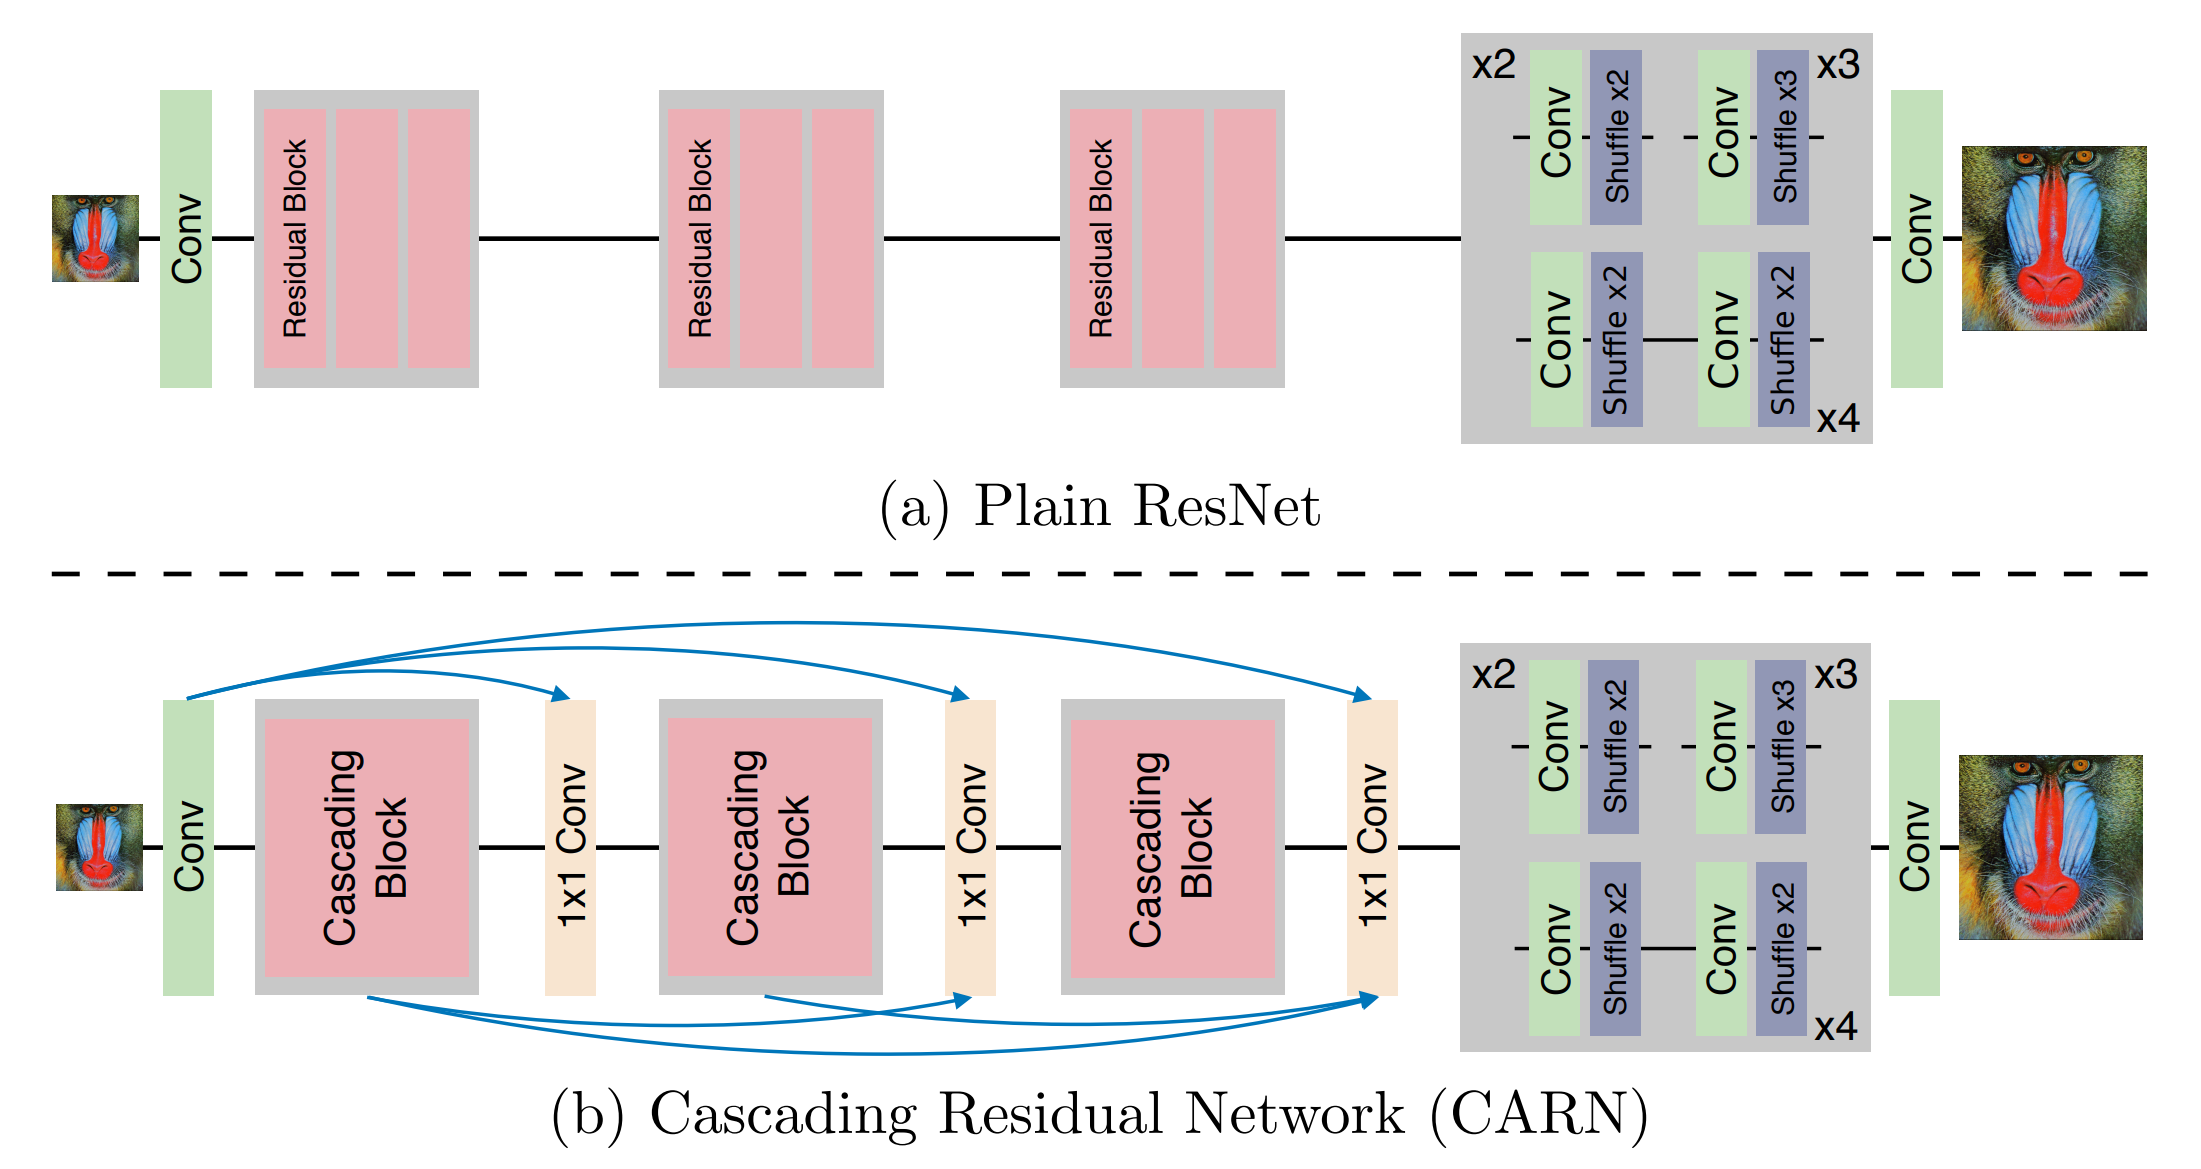
\includegraphics[width=1\linewidth]{cvpr21/CARN.jpg}
\end{center}
   \caption{(a) the plain ResNet model, (b) CARN model which the global cascading connection is indicated by the blue arrows.}
\label{CARN}
\end{figure*}


\section{Methodology}

For the super-resolution task, we propose two novel models: CARN and CARN-M. CARN is designed for good performance and CARN-M is an extension based on CARN for high efficiency.

\begin{figure}
\begin{center}
%\fbox{\rule{0pt}{2in} \rule{.9\linewidth}{0pt}}
    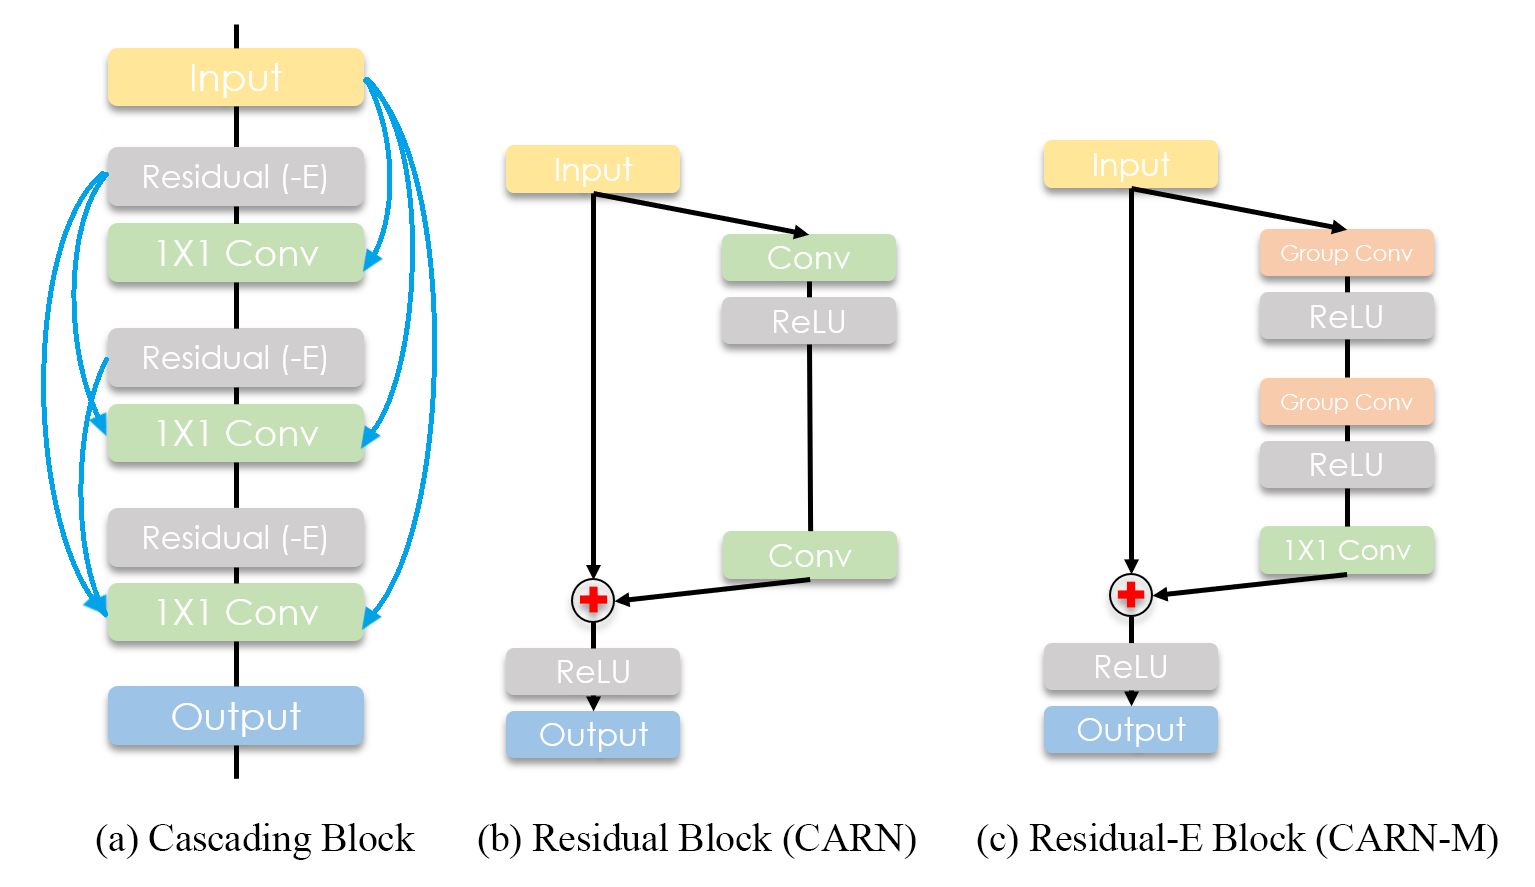
\includegraphics[width=1\linewidth]{cvpr21/blocks.png}
\end{center}
   \caption{(a) Cascading block. (b) Residual block used in CARN model. (c) Residual-E block used in CARN-M model.}
\label{blocks}
\end{figure}

\subsection{Cascading Residual Network}

Inspired by FSRCNN \cite{r5}, CARN takes LR images as input and outputs HR images restored by SR. As shown in Figure \ref{CARN} \cite{r1}, the design of the middle part of the CARN model is based on the ResNet \cite{r6}, with the residual blocks in ResNet replaced by cascading blocks. For the three cascading blocks, before entering each cascading block, the output of the previous cascading block must be fused and compressed with a 1x1 convolution kernel. There are three residual blocks in each cascading block, and the three residual blocks have the similar structure with the cascading block. Figure \ref{blocks} (a) and (b) shows the detailed block structures of CARN. This structure combines the features of multiple layers and behaves as multi-level shortcut connections, which can learn multi-level representations and the information transmission is efficient \cite{r1}. 



\subsection{Efficient Cascading Residual Network}

CARN-M is similar with CARN but more efficient. The main difference of CARN-M and CARN is that CARN-M uses the efficient residual (residual-E) block as shown in Figure \ref{blocks} (c). The residual-E block is similar with MobileNet \cite{r13}, but instead of depthwise convolution, residual-E uses group convolution. The residual-E block consists of two group convolutions followed by a 1×1 convolution layer. Group convolution allows the model to be balanced between performance and efficiency by adjusting the size of the groups.  

\section{Experiments} 

\subsection{Dataset}

Following \cite{r1}, we used DIV2K \cite{r7} dataset to train the model. It contains 800 training images, 100 validation images and 100 test images, the types of images are also rich. We also used Set5 \cite{r8}, Set14 \cite{r9}, B100 \cite{r10} and Urban100 \cite{r11} for testing and visualizing. Given that most of the pictures in the above data set are natural images, we also collected a dataset which contains only unnatural image to verify the performance of the model on unnatural images. The images in this dataset are from Pixabay with Pixabay License. 
\begin{figure*}
\begin{center}
%\fbox{\rule{0pt}{2in} \rule{.9\linewidth}{0pt}}
    \includegraphics[width=0.5\linewidth]{cvpr21/exp.png}
\end{center}
   \caption{SR results with X4 scale, 600000 steps}
\label{exp}
\end{figure*}

\begin{table*}[htbp] 
\caption{CARN and CARN-M performance on different datasets. Red figures are the highest PSNR/SSIM for this dataset on this scale while the blue figures are the second highest.}
\centering
\begin{tabular}{ccccc} 
    \toprule
    Scale & Dataset & LR (PSNR/SSIM)& CARN (PSNR/SSIM) & CARN-M (PSNR/SSIM)\\ 
    \midrule
    \multirow{5}[X2]{}
     & B100 & 27.37/0.8110 & \textcolor{blue}{30.02/0.8939} & \textcolor{red}{30.56/0.8985} \\
     & Urban100 & 24.53/0.8061 & \textcolor{red}{30.28/0.9232} & \textcolor{blue}{29.64/0.9163} \\ 
     & Set5 & 30.44/0.8982 & \textcolor{red}{35.61/0.9494} & \textcolor{blue}{35.32/0.9473} \\
     & Set14 & 27.32/0.8264 & \textcolor{red}{31.23/0.9036} & \textcolor{blue}{31.02/0.9009} \\
     & Unnatural & 25.50/0.7834 & \textcolor{blue}{25.76/0.8063} & \textcolor{red}{25.82/0.8080} \\
    \midrule
    \multirow{5}[X3]{}
     & B100 & 25.47/0.7170 & \textcolor{red}{27.73/0.8066} & \textcolor{blue}{27.57/0.8033} \\
     & Urban100 & 22.57/0.7114 & \textcolor{red}{26.50/0.8462} & \textcolor{blue}{26.01/0.8354} \\ 
     & Set5 & 27.80/0.8347 & \textcolor{red}{32.23/0.9125} & \textcolor{blue}{31.95/0.9096} \\
     & Set14 & 25.20/0.7395 & \textcolor{red}{28.14/0.8275} & \textcolor{blue}{27.91/0.8233} \\
     & Unnatural & 24.43/0.7267 & \textcolor{blue}{25.09/0.7764} & \textcolor{red}{25.20/0.7771} \\
    \midrule
    \multirow{5}[X4]{}
     & B100 & 24.24/0.6359 & \textcolor{red}{26.26/0.7336} & \textcolor{blue}{24.63/0.6653} \\
     & Urban100 & 21.25/0.6248 & \textcolor{red}{24.55/0.7793} & \textcolor{blue}{23.44/0.7305} \\ 
     & Set5 & 25.86/0.7639 & \textcolor{red}{30.12/0.8764} & \textcolor{blue}{29.84/0.8709} \\
     & Set14 & 23.72/0.6584 & \textcolor{red}{26.50/0.7645} & \textcolor{blue}{26.27/0.7595} \\
     & Unnatural & 23.56/0.6788 & \textcolor{red}{24.47/0.7382} & \textcolor{blue}{23.92/0.7224} \\
    \bottomrule
\label{com}
\end{tabular}
\end{table*}

\begin{figure*}[ht]
\begin{center}
%\fbox{\rule{0pt}{2in} \rule{.9\linewidth}{0pt}}
    \includegraphics[width=0.75\linewidth]{cvpr21/unnatural.png}
\end{center}
   \caption{Some sampels from unnatural dataset}
\label{unnatural}
\end{figure*}

\subsection{Evaluation}

Following \cite{r1}, we used two commonly used metrics to quantify the results: Peak Signal-to-Noise Ratio (PSNR) and Structural Similarity index (SSIM) \cite{r12}. At the same time, we also compare the results based on subjective judgments. 

\subsection{Initial Results}

We trained the CARN model and CARN-M model using DIV2K dataset. Due to device limitation, we trained the model for 150000 steps. The patch size and batch size are both 64, and the loss function is L1 loss. (Missing CARN-M) 

We tested the trained models on datasets Set14, B100 and Urban100, and used the built-in method of scikit-image SciKit library to calculate PSNR and SSIM. The results are shown as Figure 3. We also tried the model provided by the author, whoever the result is different with ours. In our results, the overall PSNR and SSIM are lower, even for the original bicubic images. This may be because we used a different method to calculate the PSNR and SSIM. However, both PSNR and SSIM have been greatly improved.  

We also tested the speed of the two model. Our test platform has an Intel i7-8750H CPU and a Nvidia 1050Ti GPU. Running the CARN-M model to process x4 scale of Urban100 dataset costed 75.59s while CARN costed 79.67s. On B100 dataset CARN costed 20.16s. However, CARN-M model uses fewer computing resources compared with CARN model.

\subsection{Performance on unnatural images}

We used the DIV2K data set as the training set. We tested the performance of the model on the B100, Urban100, Set14 and Set5 datasets. The images in DIV2K are all natural images, so we collected an unnatural image dataset (Unnatural) and verified the performance of the models on unnatural image SR task.  

Table \ref{com} shows the average PSNR and SSIM of the test datasets. In most cases, CARN performs better than CARN-M. Overall, CARN and CARN-M both improved the average PSNR and average SSIM on each data set and each scale. However, the PARN/SSIM improvement of CARN and CARN-M on the unnatural data set is not as good as the B100, Urban100 and Set5 data sets with only natural images, and the Set14 data set with only one unnatural image. Figure \ref{unnatural} shows some examples of x4 scale results for Unnatural dataset. For some images, the PSNR of some SR images is even lower than that of LR images, such as img014. However, the SSIM for all the images are improved. Subjectively, img014 has a lot of lines and textures. Although the SR image looks clearer, the lines and textures do not match the HR image very well. CARN and CARN-M have unstable performance on unnatural images, but they perform well in improving SSIM. Adding unnatural images in the training set may improve performance in unnatural images.

\begin{table*}[hb] 
\caption{Comparison of L1, MSE, SmoothL1 loss function on X4 scale}
\centering
\begin{tabular}{ccccc} 
    \toprule
     Dataset & LR (PSNR/SSIM) & L1 (PSNR/SSIM) & MSE (PSNR/SSIM) & SmoothL1 (PSNR/SSIM)\\ 
    \midrule
    Set5 & 25.86/0.7639 & \textcolor{red}{29.87/0.8713} & 29.79/0.8696 & 29.75/0.8704 \\
    \midrule
    Set14 & 23.72/0.6584 & \textcolor{red}{26.32/0.7609} & 26.32/0.7591 & 26.27/0.7593 \\
    \midrule
    Urban100 & 21.25/0.6248 & \textcolor{red}{24.24/0.7694} & 24.24/0.7671 & 24.23/0.7681\\
    \midrule
    B100 & 24.24/0.6359 & \textcolor{red}{26.12/0.7308} & 26.12/0.7296 & 26.10/0.7299 \\
    \midrule
    Unnatural & 23.56/0.6788 & \textcolor{red}{24.34/0.7367} & 24.34/0.7309 & 24.27/0.7331 \\
    \bottomrule
\label{loss}
\end{tabular}
\end{table*}

\subsection{Compare different loss function}

We tested different loss functions: L1, smooth L1 and SME. Table \ref{loss} shows the x4 scale performance of CARN model with different loss functions on each dataset. L1 loss performs slightly better than SME and SmoothL1 in terms of PSNR and SSIM. As for training speed, we used the same platform as 4.3. and run CARN training for 1000 iterations. L1 took 740.00 seconds, MSE took 735.33 seconds, and SmoothL1 took 749.32 seconds. Overall, these three loss functions have little effect on performance. 



\section{Conclusion}

We reproduced the CARN and CARN-M network models. We trained the model using the DIV2K dataset and compared the performance of CARN and CARN-M on B100, Urban100, Set14, Set5 and an unnatural image dataset collected by us. Overall, the performance of CARN is usually better than CARN-M, while CARN-M costs fewer computing resources than CARN. We found that the CARN and CARN-M models show good versatility on natural images, but they are unstable on unnatural images. At the same time, we explored the impact of L1, MSE, and SmoothL1 loss functions on model training and performance, and found that the model performs better when using the L1 loss function, but the difference is very small.  

Going forward, we plan to add unnatural images and more types of natural images to the training set to enhance the versatility and performance of the model. Moreover, we plan to apply this network to video SR tasks and consider the time correlation of multiple frames to enhance network performance. 

%=============================
%\subsection*{Reference}

%\small {
%[1] Ahn, N., Kang, B., &amp; Sohn, K.-A. (2018). Fast, accurate, and lightweight super-resolution with cascading residual network. Computer Vision – ECCV 2018, 256–272. \url{https://doi.org/10.1007/978-3-030-01249-6_16}

%[2] Tong, T., Li, G., Liu, X., &amp; Gao, Q. (2017). Image super-resolution using dense skip connections. 2017 IEEE International Conference on Computer Vision (ICCV). \url{https://doi.org/10.1109/iccv.2017.514}

%[3] Lim, B., Son, S., Kim, H., Nah, S., &amp; Lee, K. M. (2017). Enhanced deep residual networks for single image Super-Resolution. 2017 IEEE Conference on Computer Vision and Pattern Recognition Workshops (CVPRW). \url{https://doi.org/10.1109/cvprw.2017.151}

%[4] Zhang, Y., Tian, Y., Kong, Y., Zhong, B., &amp; Fu, Y. (2021). Residual dense network for image restoration. IEEE Transactions on Pattern Analysis and Machine Intelligence, 43(7), 2480–2495. \url{https://doi.org/10.1109/tpami.2020.2968521}

%[5] Dong, C., Loy, C. C., &amp; Tang, X. (2016). Accelerating the super-resolution convolutional neural network. Computer Vision – ECCV 2016, 391–407. \url{https://doi.org/10.1007/978-3-319-46475-6_25}

%[6] He, K., Zhang, X., Ren, S., &amp; Sun, J. (2016). Deep residual learning for image recognition. 2016 IEEE Conference on Computer Vision and Pattern Recognition (CVPR). \url{https://doi.org/10.1109/cvpr.2016.90}

%[7] Agustsson, E., &amp; Timofte, R. (2017). NTIRE 2017 Challenge on Single Image Super-resolution: Dataset and study. 2017 IEEE Conference on Computer Vision and Pattern Recognition Workshops (CVPRW). \url{https://doi.org/10.1109/cvprw.2017.150}

%[8] Bevilacqua, M., Roumy, A., Guillemot, C., &amp; Morel, M.-line A. (2012). Low-complexity single-image super-resolution based on nonnegative neighbor embedding. Procedings of the British Machine Vision Conference 2012. \url{https://doi.org/10.5244/c.26.135}

%[9] Jianchao Yang, Wright, J., Huang, T. S., &amp; Yi Ma. (2010). Image super-resolution via sparse representation. IEEE Transactions on Image Processing, 19(11), 2861–2873. \url{https://doi.org/10.1109/tip.2010.2050625}

%[10] Martin, D., Fowlkes, C., Tal, D., &amp; Malik, J. (n.d.). A database of human segmented natural images and its application to evaluating segmentation algorithms and measuring ecological statistics. Proceedings Eighth IEEE International Conference on Computer Vision. ICCV 2001. \url{https://doi.org/10.1109/iccv.2001.937655}

%[11] Huang, J.-B., Singh, A., &amp; Ahuja, N. (2015). Single Image Super-resolution from transformed self-exemplars. 2015 IEEE Conference on Computer Vision and Pattern Recognition (CVPR). \url{https://doi.org/10.1109/cvpr.2015.7299156}

%[12] Wang, Z., Bovik, A. C., Sheikh, H. R., &amp; Simoncelli, E. P. (2004). Image quality assessment: From error visibility to structural similarity. IEEE Transactions on Image Processing, 13(4), 600–612. \url{https://doi.org/10.1109/tip.2003.819861}

%[13] A.G. Howard, M. Zhu, B. Chen, D. Kalenichenko, W. Wang, T. Weyand, M. Andreetto and H. Adam. Mobilenets: Efficient convolutional neural networks for mobile vision applications. arXiv vol.1704.04861 2017. 
%}

\small {
\bibliographystyle{ieee_fullname.bst}
\bibliography{fsl.bib}

}
%=========================================

\section*{Personal Reflection}

\section*{Confidential Peer Review}

In doing this project, to the best of my judgement, I confirm that Ziyang mainly contributed to similarity matrix construction, Nystrom algorithm implementation, related part report writing and integration, and his overall contribution is about 50\%. Jawward was responsible for K-means algorithm, the IDD-lite’s semantic labeling results and related part report writing, and his contribution counts about 30\% of the total project workload. Thanks to my teammate Ziyang, he was extremely responsible for completing those most important tasks. Also thanks to Jawward for his responsibility on his work. All works that have been done realized the overall completion of this project.

\end{document}
